\documentclass[12pt,a4paper]{article}
% AUTHOR: Rafael Belchior
% Thanks to Prof. RUI SANTOS CRUZ for providing the template
%
\usepackage{helvet} 
\renewcommand{\familydefault}{\sfdefault}
\usepackage{a4wide}
\usepackage{ucs}
\usepackage[utf8x]{inputenc}
\usepackage{amsthm}
\usepackage{amsmath}
\usepackage{minted}


\theoremstyle{definition}
\newtheorem{definition}{Definition}[section]
%%%%%%%%%%%%%%%%%%%%%%%%%%%%%%%%%%%%%%%%%%%%%%%%%%%%%%%%%%%%%%%%%%%%%%%%%%%%%%%%%%%
% SELECT ONE OF THE FOLLOWING PACKAGES FOR THE LANGUAGE 
\usepackage[english]{babel}
% \usepackage[portuges]{babel}
%%%%%%%%%%%%%%%%%%%%%%%%%%%%%%%%%%%%%%%%%%%%%%%%%%%%%%%%%%%%%%%%%%%%%%%%%%%%%%%%%%
\usepackage{subfig}
\usepackage{graphicx}
\usepackage{hyperref}
\usepackage{cite}
\usepackage[absolute]{textpos}
\usepackage{tabularx} 
\usepackage{tabulary}                 
\usepackage{fancyhdr}
\usepackage[table]{xcolor}
\pagestyle{fancy}
\headsep=50pt
\setlength{\headheight}{50pt}
\usepackage{listings}
\usepackage{minted}
\definecolor{LightGray}{rgb}{0.95, 0.95, 0.95}
\definecolor{darkblue}{rgb}{0.0,0.0,0.6}
\definecolor{editorOcher}{rgb}{1, 0.5, 0}

% Clever Referencing of document parts
\usepackage{cleveref}

\lstdefinestyle{commandline} {%
language={[WinXP]command.com},
breaklines=true,
%aboveskip=\baselineskip,
belowskip=\baselineskip,
showstringspaces=false,
backgroundcolor=\color{LightGray},
basicstyle=\small\color{black}\ttfamily,
showstringspaces=false,
keywordstyle=\color{cyan}\bfseries,
stringstyle=\color{cyan}\ttfamily,
commentstyle=\color{green}\itshape,
moredelim=[s][\color{blue}\bfseries]{C:}{\>}
}

\lstdefinestyle{Bash} {%
language=bash,
breaklines=true,
belowskip=\baselineskip,
backgroundcolor=\color{LightGray},
showstringspaces=false,
keywordstyle=\color{black}\bfseries,
basicstyle=\small\color{black}\ttfamily,
stringstyle=\color{editorOcher}\ttfamily,
commentstyle=\color{cyan}\itshape,
otherkeywords={xcode-select, mkdir,rm},
moredelim=[s][\color{red}]{~$},
literate={~} {$\sim$}{1}
}
%%%%%%%%%%%%%%%%%%%%%%%%%%%%%%%%%%%%%%%%%%%%%%%%%%%%%%%%%%%%%%%%%%%%%%%%%%%%%%%%%%%
% PLEASE FILL THE ADEQUATE DATA IN THE TABLE REPLACING
% THE VALUES EXEMPLIFIED
\lhead{}
{\renewcommand{\arraystretch}{1.1}
\fancyhead[C]{\begin{tabularx}{1.0\textwidth}{|l|X|l|l|}
\hline 
% In the following line change Course Name: PPIII, PPB
\textbf{EB 20/21} & \textbf{Enterprise Blockchain Technologies} & \textbf{Number:}  &  3 \\
\hline
% In the following line insert your Name and IST ID
\multicolumn{2}{|l|}{Module I - Introduction} & \textbf{Issue Date:}  &  - \\ 
\hline
% In the following line insert the Activity CODE and Title (abridged)
%\textbf{WP n.} (99) & (Subject) & \textbf{Group:} & (99) \\
\multicolumn{2}{|l|}{Background: A Primer on Blockchain Technology} & \textbf{Due Date:} &  - \\ 
\hline
\end{tabularx}}
\rhead{}}

%%%%%%%%%%%%%%%%%%%%%%%%%%%%%%%%%%%%%%%%%%%%%%%%%%%%%%%%%%%%%%%%%%%%%%%%%%%%%%%%%%%
% DO NOT CHANGE THIS BLOCK
\begin{document}
\textblockorigin{-34pt}{-12pt}
\begin{textblock*}{10cm}(2cm,1cm)

\includegraphics[width=6cm]{hyperledger.png}
\end{textblock*}
%%%%%%%%%%%%%%%%%%%%%%%%%%%%%%%%%%%%%%%%%%%%%%%%%%%%%%%%%%%%%%%%%%%%%%%%%%%%%%%%%%%,sdist2017

\section*{Preliminary Notes}
This class provides background about blockchain technology. This laboratory is based on previous work elaborated by the contributors \cite{belchior2019_audits,belchior2020,belchior2019_thesis}. We recommends students to have attended Lab1 and Lab2.


%The reference section should be viewed as a ``additional readings reference'' - if you would like more information about the topic.


%%%%%%%%%%%%%%%%%%%%%%%%%%%%%%%%%%%%%%%%%%%%%%%%%%%%%%%%%%%%%%%%%%%%%%%%%%%%%%%%%%%
% YOUR TEXT STARTS HERE
%%%%%%%%%%%%%%%%%%%%%%%%%%%%%%%%%%%%%%%%%%%%%%%%%%%%%%%%%%%%%%%%%%%%%%%%%%%%%%%%%%%   

%%%%%%%%%%%%%%%%%%%%%%%%%%%%%%%%%%%%%%%%%%%%%%%%%%%%%%%%%%%%%%%%%%%%%%%%%%%%%%%%%%%

\section{A Primer on Blockchain}
We now introduce Blockchain, whereby its building blocks are rooted on Distributed Systems and Cryptography (see Lab01 and Lab02). 

%TODO motivation, use cases
%\subsection{What is Blockchain For}


\subsection{A Technical Viewpoint}
The term blockchain is generally referred to as a replicated data structure: a persistent, auditable, immutable, append-only distributed ledger. The blockchain is maintained by a group of physical machines, nodes (or peers or participants). Nodes are not trusted individually to maintain the distributed ledger; they are trusted as a group, due to their number and diversity. As long as nodes have conflicting interests, collusion between them will probably not happen: and thus the network can be considered safe. Blockchain, in fact, implements many concepts discussed in Lab01: for instance, it is a byzantine fault tolerant (or just crash fault tolerant) replicated state machine that agrees on a global state via consensus. The blockchain is secure due to a combination of decentralization and cryptograpy: transactions are aggregated in blocks, linked by the cryptographic hash of the previous block. If a participant changes a prior block, its hash will change, as well as the posterior hashes. 


Most blockchains serve as a runtime for programs called smart contracts. The execution of smart contracts is originated by transactions. Smart contracts are executed in a virtual machine, e.g., in the Ethereum Virtual Machine (EVM) in Ethereum, one of the most used blockchains. Smart contracts can abstract the representation of currency, resources, assets, access, equity, identity, collectibles,  via tokens. 

There are different types of blockchains, which can typically be categorized into permissionless blockchains and permissioned blockchains.

\subsubsection{Permissionless blockchains}
Public blockchains can be accessed and utilized by anyone with Internet access. Permissionless blockchains do not require participants to be identified to participate. We use public and permissionless as synonyms. Typically, in such networks, the participants are rewarded for supporting the ecosystem, making it self-sustainable. The first entirely decentralized digital currency, Bitcoin, is a permissionless peer-to-peer version of electronic cash, which would allow transactions to go directly from one party to the other, excluding the need for any intermediary. Bitcoin quickly gained popularity because it solved the famous double-spending problem, without the need of any central authority. 

Examples: Bitcoin, Ethereum, EOS, Ripple, IOTA.

\subsubsection{Permissioned blockchains}
Permissioned blockchains identify and associate participation right to participants. Private blockchains require credentials for participants to vizualize it. We use private and permissioned as synonyms. Private blockchains are the property of an organization or consortium of organizations. If more than one organization is included in the management of the blockchain, it is called a community or federated blockchain. A permissioned solution seems suitable for companies aiming for competitiveness that blockchain technology can offer, while protecting sensitive information. Write permissions are kept centralized to specific nodes within the organization. Therefore, a trade-off between control and decentralization exists. On a technological point of view, compared to public blockchains, there is an aggravated risk of subversion, as there are fewer participants in the network that validates transactions. Neverthesless, in practice, as the network only allows identified participants, it is easier to identify a culprit.

Examples: Hyperledger Fabric, Hyperledger Indy, Hyperledger Burrow, Hyperledger Sawtooth, R3 Corda, and Multichain.

\subsection{Comparison}
Public and private blockchains are essencially different in nature. Inside each category, blockchains are also very different: their consensus, networking, data, and application layers can differ substantially, leading to a wide-range of choices. This leads to fragmentation, where some blockchains are immature (not stable). While this can be a big problem, research in blockchain interoperability attenuates this \cite{belchior2020}. 

\begin{figure}
    \centering
    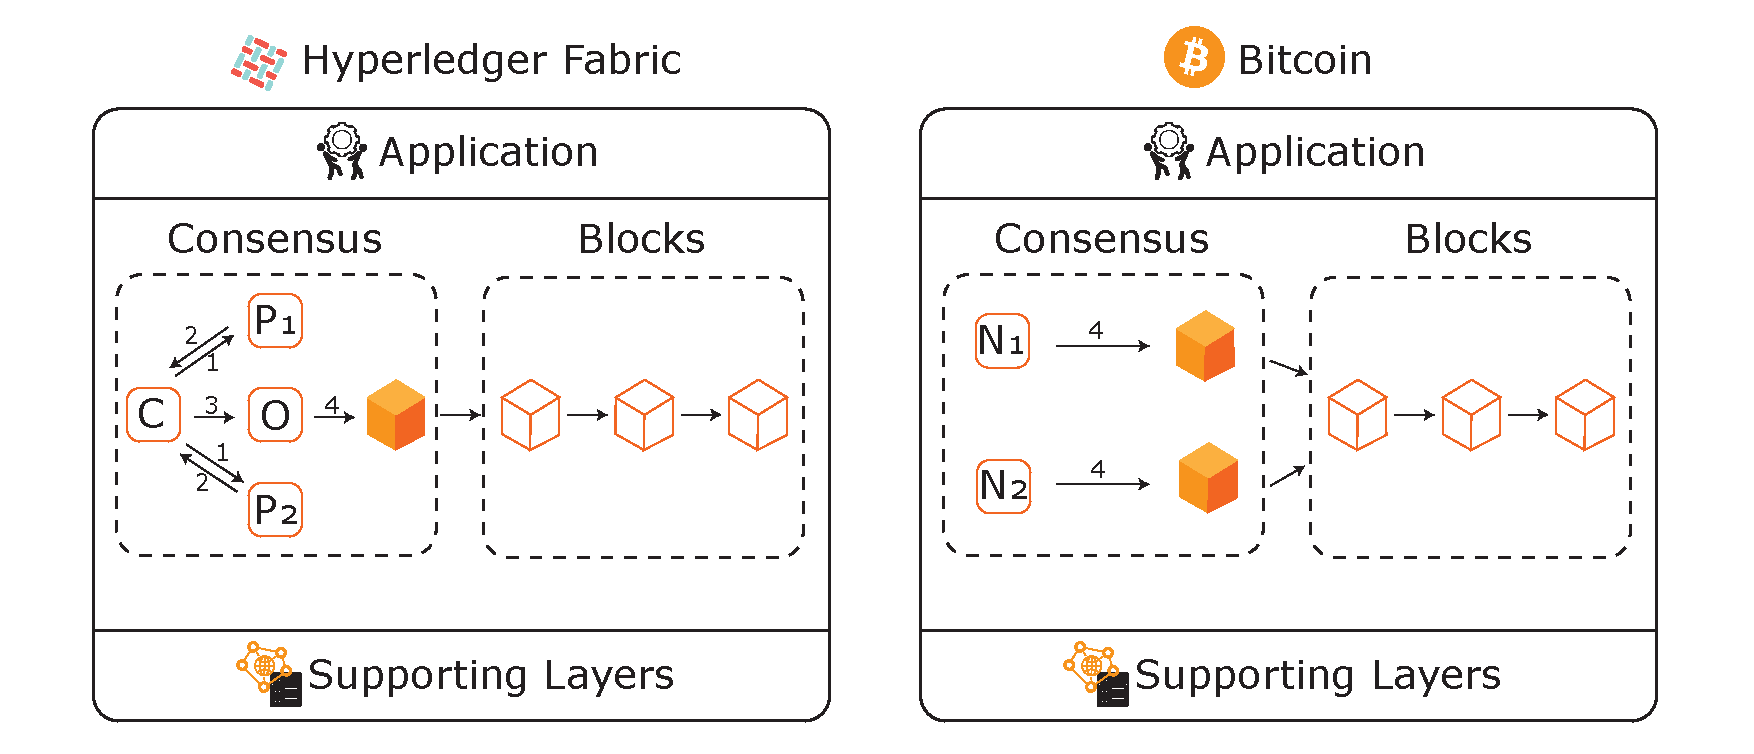
\includegraphics[scale=0.4]{figures/Fig1.pdf}
    \caption{High-level comparison of Hyperledger Fabric and Bitcoin, from \cite{belchior2020survey}}
    \label{fig:bcs}
\end{figure}

Figure \ref{fig:bcs} depicts two blockchains: Hyperledger Fabric, a permissioned blockchain; and Bitcoin, a permissionless

In Hyperledger Fabric, the consensus is based on endorsement policies. In Fabric, a client (C) sends a transaction proposal to the peer nodes (P), and obtains a signed transaction, called an endorsement (steps 1 and 2). An orderer validates the endorsements and builds a block with valid transactions, appending it to the ledger (steps 3 and 4). In Bitcoin, the consensus is based on the notion of Proof-of-Work (PoW), a cryptographic puzzle that mining nodes need to solve in order to build a valid block. This corresponds roughly to Fabric’s steps 1-3. After a node finds a solution to PoW, it then can propose a block of transactions to be appended to the ledger (step 4).


\section{Blockchain4Students}
A very reliable way to learn blockchain is to build one. Blockchain4Students is a blockchain\footnote{https://github.com/BlockChain4Students/blockchain\_node} written in the Python programming language specifically tailored to be easily understandable, and thus be a reliable basis for blockchain teaching. Let's dive deeper into the blockchain world by exploring Blockchain4Students.


\section{Hands on Blockchain}
%explain our prototype, show code

%set up blockchain with 3 nodes and setup UI


%questions on:
% node configuration
% node discovery 
% block
%
% transactions
% pow and longest chain
% attacks (submit invalid block or invalid tx) 
% extend the blockchain


\subsection{Theory \& Business}

%private vs public

\subsubsection*{Exercise 1: What is the advantage of the Blockchain being a decentralized, Peer-to-Peer system instead of a centralized one?}

\subsubsection*{Exercise 2: Consider a private blockchain running three nodes. Given that it is managed from a single organization, how do we assure decentralization?}

\subsubsection*{Exercise 3: What stops a malicious entity from being able to alter blocks in a permissionless blockchain?}

\subsubsection*{Exercise 4: What about permissioned blockchains? Can a malicious entity change in these as well?}

%Txs
\subsubsection*{Exercise 5: How does a client insert a transaction in the system?
}

\subsubsection*{Exercise 6: How do we know if a transaction was created by a client and not by a malicious node?}

%PoW

\subsubsection*{Exercise 7: Why cant permissionless blockchains use the classical Consensus algorithms and must instead rely on other forms of Consensus like Proof-Of-Work?}

\subsubsection*{Exercise 8: Why can't a node fake a result from Proof-of-Work?}

\subsubsection*{Exercise 9: Why do we want to add difficulty to the Proof-of-Work?}

\subsubsection*{Exercise 10: How does the difficulty value work in Proof-of-Work?}

%Block creation

\subsubsection*{Exercise 11: How does a node share its new block?}

\subsubsection*{Exercise 12: What are the advantages and disadvantages of sharing the chain by broadcasting the block or by verifying other chains from peer nodes?}

\subsubsection*{Exercise 13: What happens when multiple nodes mine a new block at the same time?}

\subsubsection*{Exercise 14: Why do the miners choose the longest chain to work and not a forked, smaller chain?}

\subsubsection*{Exercise 15: What happens to the other block and transactions that were created in the forked chain that was discontinued?}



\subsubsection*{Exercise 16: What if the service was already made and the payment (in the form of a transaction) disappears?}

\subsubsection*{Exercise 17: Being a Peer-to-Peer service, how does a node discover which nodes to connect to in order to join the system?}

\clearpage


\subsection{Blockchain4Students}
Consider the source code of Blockchain4Students. Start by exploring ``blockchain-data-structure'' and ```consensus'', inside the blockchain folder.


\subsubsection*{Exercise 1: Consider the next code fragment. What type is the Blockchain4Students blockchain? }


\begin{minted}[mathescape,
               linenos,
               numbersep=5pt,
               gobble=2,
               frame=lines,
               framesep=2mm]
               {python}
\@app.route('/register/node', methods=['POST'])
def register_peer_node():
    node_address = request.get_json()["node_address"]

    response = {
        'message': 'Node added',
        'total_nodes': list(blockchain.peer_nodes),
    }
    blockchain.register_node(node_address)
    return json.dumps(response), 200

\end{minted}



\subsubsection*{Exercise 2: We give rewards right after a block is mined. What is the problem with this approach?}

\subsubsection*{Exercise 3: Each Transaction include the ID from the node that created it. Why is this information necessary?}

\subsubsection*{Exercise 4: When a transaction request arrives to the node, it signs it with its own private key. What is the possible attack with this approach?}

\subsubsection*{Exercise 5: When a node first connects, it contacts a discovery node to find other peers in the blockchain. Although this method is possible, why is it not realistic to use on wider scale blockchains? }

\subsubsection*{Exercise 6: When the node obtains a valid chain bigger than its own, it discards its own chain for the bigger one. Why? }

\subsubsection*{Exercise 7: With our current implementation, when a node joins he is not aware of any state of its peers. Add the functionality of when a node joins the system, to ask and update its own blockchain.}

%%%%%%%%%%%%%%%%%%%%%%%%%%%%%%%%%%%%%%%%%%%%%%%%%%%%%%%%%%%%%%%%%%%%%%%%%%%%%%%%%%%
% YOUR TEXT ENDS HERE
%%%%%%%%%%%%%%%%%%%%%%%%%%%%%%%%%%%%%%%%%%%%%%%%%%%%%%%%%%%%%%%%%%%%%%%%%%%%%%%%%%% 
\bibliographystyle{abbrv}
\bibliography{lab.bib}

\end{document}                             % The required last line